% Created:  Fri 01 Aug 2014 02:02 PM
% @author Josh Wainwright
% filename: analysis.tex

\section{Cluster Analysis}
\label{sec:cluster_analysis}

Once the data has been processed and a number of clusters have been identified,
they can be displayed on screen in an image to verify what was found and
perform further analysis. However, since the data that was used to find the
clusters is still held in memory at this point, it is useful to take advantage
of this and perform some immediate analysis and provide some statistics
regarding the clusters that were found.

There are two ways of conceptually viewing the clusters which will lead to
slightly different results when analysing them.

\begin{itemize}

	\item The first is to consider the boundary of the nodes of the quadtree
		that were considered to be part of a cluster to be the boundary of the
		cluster. This will mean that the actual cluster is likely to be
		slightly larger than the actual data points that it is comprised of,
		but is computationally simple to achieve, so fast, and can take into
		account any holes in the cluster.

	\item The second way is to, once the cluster has been located, discard the
		information about the nodes themselves, and simply use them to select
		the appropriate points. This results in a set of points that are all
		considered to be spatially grouped into the same cluster. From this
		set, calculations can be performed on the real data. This method is
		guaranteed to provide information that more closely represents the
		original data, though is more computationally intensive.

\end{itemize}

\subsection{Quadtree Node Analysis}
\label{sub:quadtree_node_analysis}

Here, the nodes of the quadtree that were considered part of the cluster are
considered, rather than the points that they contain.

\subsubsection{Cluster Area}
\label{ssub:cluster_area_node}

To calculate the area of the clusters, each node in each cluster is examined.
Since the size of the node must be known, it is calculated from the quadtree
code for that node. The formula is shown in Equation~\ref{eq:node-area},
\begin{align}
	a &= \frac{1}{4^{d}} \\
	a_i &= 4^{-l_i/2}, \label{eq:node-area}
\end{align}
where $a_i$ is the area of the node $i$, $d$ is the depth in the quadtree and
$l_i$ is the length of the quadtree code of that node. For every node in the
cluster, where there are $n$ nodes, this value is summed to give the total
cluster area, $A$:
\begin{align}
	A &= \sum_{i=0}^{n} a_i.
\end{align}

\subsubsection{Cluster Perimeter}
\label{ssub:cluster_perimeter_node}

Similarly to the cluster area, the perimeter is given as a fractional value of
the length of one side of the whole image, as calculated for each node from the
quadtree code, as shown in Equation~\ref{eq:node-perimeter},
\begin{align}
	p &= \frac{1}{2^{d}} \\
	p_i &= 2^{-l_i/2}, \label{eq:node-perimeter}
\end{align}
where the symbols have the same meaning as above.

However, this simply gives the length of one side of the node for any node. In
order to calculate the perimeter of the cluster, it is not enough to simply
sum these values, as for the cluster area, since not all nodes contribute to
the perimeter. Instead, for each node, it must be decided whether it
contributes to the perimeter and how much (1, 2, 3 or 4 sides), and then
increase the total perimeter by this many times the length of one side. The
total perimeter, $P$, then is given by Equation~\ref{eq:total-perimeter},
\begin{align}
	P &= \sum_{i=0}^{n} s * p_i, \label{eq:total-perimeter}
\end{align}
where $s \in \{0..4\}$. This is demonstrated in
Figure~\ref{fig:perimeter-edges} where the perimeter is simple to calculate in
case (a) as the nodes are all the same, but the size of each node must be taken
into account in case (b).

\begin{figure}[tbhp]
	\centering
	\begin{subfigure}[c]{3.5cm}
		\includegraphics[width=\textwidth]{perimeter-edges-grid.pdf}
		\caption{}\label{fig:perimeter-edges-grid.pdf}
	\end{subfigure}%
	\quad
	\begin{subfigure}[c]{3.5cm}
		\includegraphics[width=\textwidth]{perimeter-edges-quadtree.pdf}
		\caption{}\label{fig:perimeter-edges-quadtree.pdf}
	\end{subfigure}

	\caption[Perimeter size from node edge size.]{When calculating the
		perimeter of a cluster using the nodes that contribute, the size of
		each node must be taken into account. In
		case~\subref{fig:perimeter-edges-grid.pdf}, the process is simple since
		all nodes are the same size and a fractional value of 3.5 is
		calculated. For case~\subref{fig:perimeter-edges-quadtree.pdf}, the
		steps are 25 lengths of size $\rfrac{1}{8}$ and 6 lengths of size
		$\rfrac{1}{16}$ which gives the same result,
		3.5.}\label{fig:perimeter-edges}

\end{figure}

Within the cluster, \emph{holes} occur where a node, or number of nodes, is
surrounded on all sides by the same cluster. An example can be seen in
Figure~\ref{fig:kernel-options}. Unfortunately, these are included in the
calculation of the perimeter and so, where holes exist in a cluster, the actual
perimeter is slightly smaller than that calculated.

\subsubsection{Cluster Roundness}
\label{ssub:Cluster_Roundness}

A potentially useful measure of a cluster is its \emph{roundness}. This
describes the extent to which the area and perimeter of the cluster resemble a
circle. The available values of roundness are from 0, meaning a perfect line
with no area but finite perimeter, to 1, being a perfect circle. The equation
to determine roundness, Equation~\ref{eq:roundness} is defined such that it is
a unit-less ratio of area and perimeter, such that a circle has roundness 1.
The derivation of Equation~\ref{eq:roundness} is found in
Appendix~\ref{app:roundness_derivation}.

\begin{align}
	R &= \sqrt{\frac{4\pi A}{p^2}} \label{eq:roundness}
\end{align}

The clusters that are found for data sets \texttt{palm-1.txt} and
\texttt{palm-2.txt} are shown in Figure~\ref{fig:roundness}. The roundness
values for the clusters for these data are very different,
Figure~\ref{fig:roundness-long.png} has an average $R=0.350$ whereas
Figure~\ref{fig:roundness-round.png} has an average $R=0.446$.

\begin{figure}[tbhp]
	\centering
	\begin{subfigure}[b]{4.2cm}
		\fbox{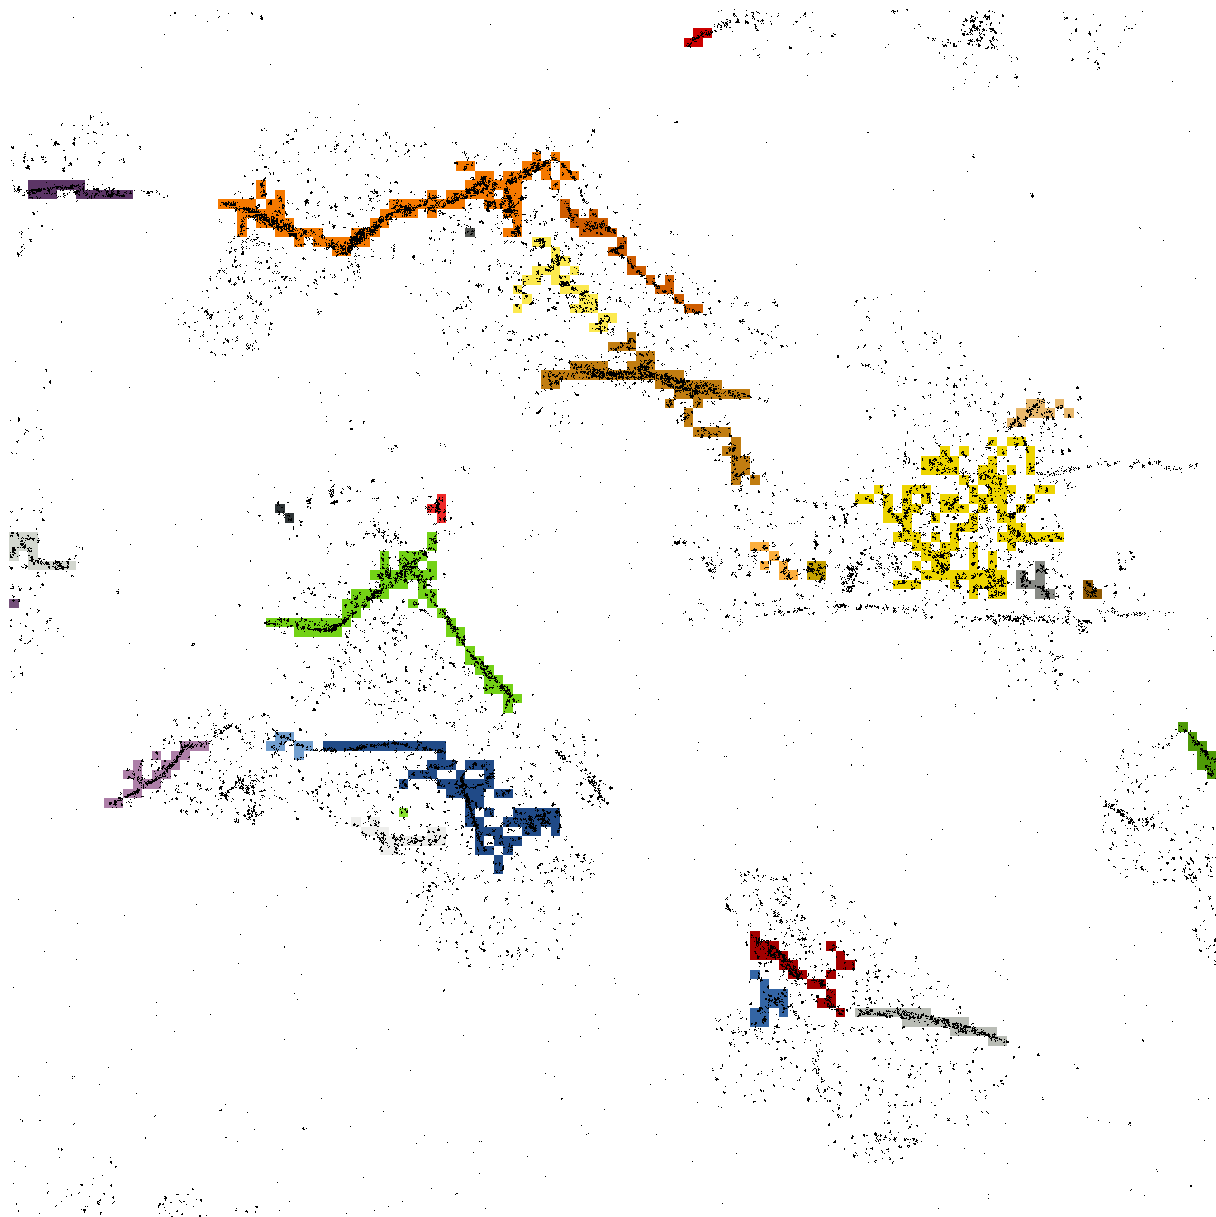
\includegraphics[width=\textwidth]{roundness-long.png}}
		\caption{}\label{fig:roundness-long.png}
	\end{subfigure}%
	\quad
	\begin{subfigure}[b]{4.2cm}
		\fbox{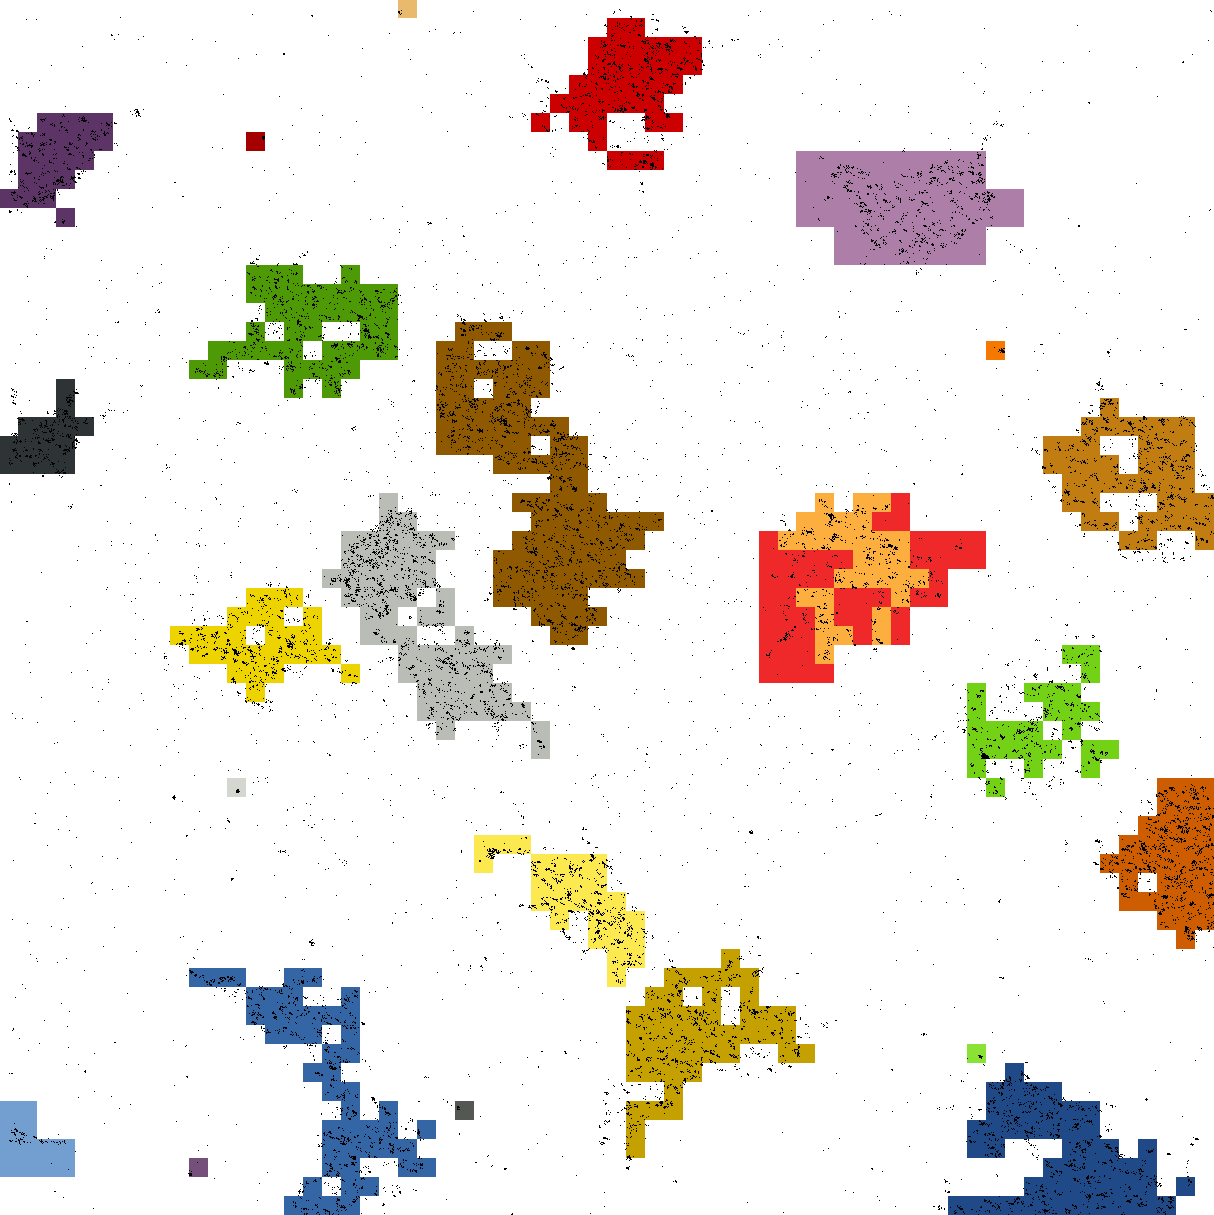
\includegraphics[width=\textwidth]{roundness-round.png}}
		\caption{}\label{fig:roundness-round.png}
	\end{subfigure}

	\caption[A comparison of roundness values.]{The general shape of the
		clusters found can be described using the roundness measure. A value
		closer to 0 means longer and thinner clusters, whereas values closer to
		1 mean clusters that are more circular.}\label{fig:roundness}
\end{figure}

\subsection{Point Analysis}
\label{sub:point_analysis}

Here, the points contained in the nodes of quadtree that were considered part
of the cluster are considered; the nodes are only used to select the correct
points.

\subsubsection{Cluster Perimeter}
\label{ssub:cluster_perimeter_point}

\subsubsection*{Convex Hull Algorithm}
\label{ssub:Convex Hull Algorithm}

There are a number of algorithms that atempt to find the bounding polygon of a
set of points. Ignoring any holes in the cluster, the perimeter of this bouding
polygon is equivalent to the perimeter of the cluster.

The simplest method of finding this bounding polygon is using the \emph{convex
hull} method\cite{barber1996quickhull}. In principle, this involves starting
with a circle far larger than the points it encloses, which is reduced in size,
without letting any point leave the shape, until only stright lines exist
between external points. The final shape can be pictured by imaginging each of
the points as being represented by a nail in a piece of wood. The convex hull
algorithm then calculates the shape that would be produced if an elastic band
were streched around these nails.

The major disadvantage of this algorithm is that, as the name suggest, the
final shape consists only of convex angles, meaning that the actual shape of
the perimeter of the points may be lost, as shown in
Figure~\ref{fig:convex-hull}.

\begin{figure}[tbhp]
	\centering
	\includegraphics[width=5cm]{convex-hull.pdf}

	\caption[Convex versus concave hull algorithms.]{Convex versus concave hull
		algorithms. The red line shows the convex hul found for this set of
		points, which misses much of the detail and will report the area as
		being significantly above its actual value. The blue line is the
		concave hull found.}\label{fig:convex-hull}
\end{figure}

\subsubsection*{Concave Hull Algorithm}
\label{ssub:Concave Hull Algorithm}

An alternative to the convex hull algorithm is the slightly more complex
\emph{concave} hull algorithm\cite{moreira2007concave}. Instead of simply
finding the outermost shape that will enclose all of the points, the concave
hull algorithm finds that shape that fits the outer boundary of the points more
closely. The steps involved are listed below.

\begin{enumerate}
	\item The algorithm looks at the distance to each of the nearest $n$
		points, where $n$ is specified beforehand.
	\item From these possibilities, it chooses the closest to be added to the
		``hull''.
	\item The new line segment that would be added by joining the existing hull
		to the new point is examined to ensure that it does not cross the
		existing hull at all.
	\item If it does cross, this point is removed as a possibility of being a
		part of the hull and the next nearest point is checked.
	\item When the initial starting point is reached again, the algorithm will
		have generated a closed loop joining a number of points togther.
	\item This closed loop is checked to ensure that all points lie either on
		the hull or are enclosed within it.
	\item If there are any points that fall outside the hull, the results are
		abandoned and the algorithm is re-run with the number of neighbours to
		check, $n$, incremented by one.
	\item When a hull is found that encloses all points, the algorithm
		terminates.
\end{enumerate}

\cite{lee2002polygonization}

\cite{estivill2000autoclust}

\cite{xia2006border}

% TODO mention delaunay triangulation
\cite{lee1980two}

\subsubsection{Cluster Area}
\label{ssub:cluster_area_point}

Once the perimeter hull of the cluster of points has been identified, it is
simple to calculate the area enclosed by that cluster from the hull. Since the
hull consists only of straight lines connecting single points, the area can be
calculated by splitting the polygon into regular triangles, and finding each of
their areas individually. The area of the whole cluster is then given by the
sum of these areas. An algorithm for calculating the area of the irregular
polygon produced with this method is shown in Listing~\ref{lst:polygon-area}.

\begin{lstlisting}[caption={Code to find the area of an irregular polygon.
	Adapted from~\cite{finley2006poly}}, label=lst:polygon-area]
	public |polygonArea(points, numPoints)| {

		area = 0;
		j = numPoints - 1;

		/* Sum the area contained between each pair of points and the y-axis on the right hand side of the shape and subtract the area between pairs of points and the y-axis on the left hand side. */
		for (i=0; i < numpoints; i++) {
			area += (points[j].getX() + points.[i].getX()) *
		        	(points[j].getY() - points.[i].getY());
			j = i;
		}
		return area/2;
	}
\end{lstlisting}
